\documentclass[11pt,a4paper]{article}

\usepackage[T1]{fontenc}
\usepackage[utf8]{inputenc}
\usepackage{lmodern}
\usepackage{microtype}
\usepackage[a4paper,margin=22mm,headheight=14pt]{geometry}
\usepackage{amsmath,amssymb}
\usepackage{booktabs,tabularx,array}
\usepackage{enumitem}
\usepackage{xcolor}
\usepackage{tikz}
\usetikzlibrary{arrows.meta,positioning,calc,fit,shapes.geometric}
\usepackage[most]{tcolorbox}
\usepackage{fancyhdr}
\usepackage{titlesec}
\usepackage{hyperref}
\usepackage{ragged2e}

\definecolor{navy}{RGB}{29,59,91}
\definecolor{blue}{RGB}{53,105,151}
\definecolor{sky}{RGB}{238,246,252}
\definecolor{mint}{RGB}{239,248,243}
\definecolor{sand}{RGB}{252,248,235}
\definecolor{rose}{RGB}{252,241,241}
\definecolor{violet}{RGB}{246,242,250}
\definecolor{ink}{RGB}{50,50,50}
\definecolor{midgray}{RGB}{105,105,105}
\definecolor{lightgray}{RGB}{247,248,249}

\hypersetup{
  colorlinks=true,
  linkcolor=navy,
  urlcolor=navy,
  pdftitle={Computational Identity and Computational Functionalism: A Conceptual Guide},
  pdfsubject={A problem-driven theory of computational identity followed by structural constraints on computational functionalism of consciousness}
}

\pagestyle{fancy}
\fancyhf{}
\fancyhead[L]{\small Computational Identity: Conceptual Guide}
\fancyhead[R]{\small \thepage}
\renewcommand{\headrulewidth}{0.3pt}

\titleformat{\section}{\Large\bfseries\color{navy}}{\thesection}{0.7em}{}
\titleformat{\subsection}{\large\bfseries\color{navy}}{\thesubsection}{0.6em}{}

\setlist[itemize]{topsep=4pt,itemsep=2.3pt,parsep=1pt,leftmargin=1.45em}
\setlist[enumerate]{topsep=4pt,itemsep=3pt,parsep=1pt,leftmargin=1.65em}
\setlength{\parindent}{0pt}
\setlength{\parskip}{5.2pt}

\newtcolorbox{thesisbox}[1][]{
  enhanced,breakable,colback=sand,colframe=navy,boxrule=0.9pt,
  arc=1.5mm,left=2.5mm,right=2.5mm,top=2mm,bottom=2mm,
  title={Central thesis},fonttitle=\bfseries,#1
}

\newtcolorbox{conceptbox}[1][]{
  enhanced,breakable,colback=sky,colframe=blue,boxrule=0.7pt,
  arc=1.4mm,left=2.3mm,right=2.3mm,top=1.7mm,bottom=1.7mm,
  title={Concept forced by the example},fonttitle=\bfseries,#1
}

\newtcolorbox{consequencebox}[1][]{
  enhanced,breakable,colback=mint,colframe=navy,boxrule=0.75pt,
  arc=1.4mm,left=2.3mm,right=2.3mm,top=1.7mm,bottom=1.7mm,
  title={Consequence},fonttitle=\bfseries,#1
}

\newtcolorbox{cautionbox}[1][]{
  enhanced,breakable,colback=rose,colframe=ink,boxrule=0.65pt,
  arc=1.4mm,left=2.3mm,right=2.3mm,top=1.6mm,bottom=1.6mm,
  title={What not to conclude},fonttitle=\bfseries,#1
}

\newtcolorbox{definitionbox}[1][]{
  enhanced,breakable,colback=violet,colframe=navy,boxrule=0.7pt,
  arc=1.4mm,left=2.3mm,right=2.3mm,top=1.6mm,bottom=1.6mm,
  title={Working definition},fonttitle=\bfseries,#1
}

\newtcolorbox{takeawaybox}[1][]{
  enhanced,breakable,colback=lightgray,colframe=midgray,boxrule=0.65pt,
  arc=1.4mm,left=2.2mm,right=2.2mm,top=1.5mm,bottom=1.5mm,
  title={Takeaway},fonttitle=\bfseries,#1
}

\newtcolorbox{principlebox}[1][]{
  enhanced,breakable,colback=mint,colframe=blue,boxrule=0.85pt,
  arc=1.5mm,left=2.4mm,right=2.4mm,top=1.8mm,bottom=1.8mm,
  title={Constraint on an admissible functionalism},fonttitle=\bfseries,#1
}

\newtcolorbox{stressbox}[1][]{
  enhanced,breakable,colback=rose,colframe=navy,boxrule=0.8pt,
  arc=1.5mm,left=2.4mm,right=2.4mm,top=1.8mm,bottom=1.8mm,
  title={Stress test},fonttitle=\bfseries,#1
}

\newcounter{thought}
\newenvironment{thoughtbox}[1]{%
  \refstepcounter{thought}%
  \begin{tcolorbox}[
    enhanced,breakable,
    colback=white,colframe=navy,boxrule=0.85pt,
    arc=1.7mm,left=2.8mm,right=2.8mm,top=2.2mm,bottom=2.0mm,
    borderline west={2.2pt}{0pt}{blue},
    title={\large\bfseries Thought experiment \thethought: #1},
    fonttitle=\bfseries,coltitle=navy,
    attach boxed title to top left={xshift=2mm,yshift=-2mm},
    boxed title style={colback=sky,colframe=blue,boxrule=0.55pt,arc=1.2mm},
    before skip=9pt,after skip=10pt
  ]
}{\end{tcolorbox}}

\newcommand{\scene}{\medskip\textbf{Setup.} }
\newcommand{\failure}{\medskip\textbf{What goes wrong.} }
\newcommand{\lesson}{\medskip\textbf{What the example forces us to add.} }
\newcommand{\question}{\medskip\textbf{Question exposed.} }

\begin{document}

\begin{center}
{\LARGE\bfseries\color{navy} Computational Identity and Computational Functionalism}\\[2mm]
{\Large A problem-driven conceptual guide}\\[3mm]
{\large From thought experiments to a disciplined theory architecture}\\[3mm]
{\small August 2026}
\end{center}

\begin{thesisbox}[title={What this note does}]
This note has two deliberately separated parts.

\textbf{Part I develops a theory of computational identity from a series of diagnostic failure cases.} Arbitrary state relabeling, function-versus-algorithm, local abstraction, non-linear granularity, the stone-factorization challenge, ambiguity about causal participation, and the split between actual and counterfactual organization jointly motivate a picture in which physical episodes support structured spectra of admissible computational abstractions grounded in coherent value representation and actual computational provenance.

\textbf{Part II applies that computational ontology to computational functionalism.} It formulates constraints on the \emph{form} of a consciousness-making computational property: its required invariances, the proper role of counterfactual structure, and the priority of the process actually instantiated over unrealized alternatives.
\end{thesisbox}

\section{The problems that force the theory}

\begin{thoughtbox}{The relabeling trick}
\scene Imagine that a computation is represented only by a finite sequence of internal states: first state $A$, then $B$, then $C$, and so on. Now take any physical object whose global microstate changes over time -- a stone, a turbulent fluid, a processor, a brain. Record a sequence of distinct snapshots.

A dictionary can now be invented after the fact: call the first physical snapshot ``computational state $A$,'' the second ``state $B$,'' the third ``state $C$,'' and so forth.

\failure If a successful computational implementation requires only that a sequence of physical states can be put in correspondence with a sequence of abstract states, almost any sufficiently rich history can be made to implement almost any finite run. The alleged computation is doing no explanatory work. The dictionary is doing all of it.

\lesson A realized computation cannot be represented as a bare sequence of atomic global states. The representation must preserve some of the internal organization of the actual process: which events occurred, which value-bearing tokens were present, where those tokens were routed, which events consumed them, what new tokens were produced, and which parts of the process were independent.

There is a second constraint. The interpretation of values cannot be reinvented at every instant. If one physical carrier is read as the abstract value $7$ here and the same type of carrier is read as $23$ later merely because that makes the desired trajectory fit, the relabeling trick has returned in local form. What is required is not one unique physical code for the entire system, but a \textbf{coherent representation scheme}: a stable family of local or typed decoding rules that can be reused across the episode and does not depend on knowing the completed trajectory. The rule may itself depend on an explicitly represented mode or local context; what is excluded is an ad hoc change of interpretation indexed only by where one happens to be in the desired history.

\begin{conceptbox}
The first primitive object should be an \textbf{actual valued computational provenance structure}, not a state sequence. A run has internal organization, and its value interpretation must be trajectory-independent and reusable. The order ``first, second, third'' is only one projection of that richer structure.
\end{conceptbox}
\end{thoughtbox}

\begin{thoughtbox}{The stationary decoder that still fits anything}
\scene Strengthen the previous proposal: one fixed local decoder must be used throughout the episode. Now suppose that every exact carrier microstate encountered during the finite run is unique. None of the physical values ever repeats exactly.

\failure A single stationary lookup rule can still be defined after the fact, assigning each unique carrier state whatever abstract value the target trajectory requires. The decoder no longer mentions time, yet the completed answer remains hidden in its graph. Stationarity blocks contradictory reuse of one carrier state; it does not by itself block arbitrary labeling of states seen only once.

\lesson Coherence is necessary but not sufficient. The eligible carrier variables and decoder family must be fixed independently of the desired computation. Useful constraints include physically natural coarse variables, locality, bounded descriptive complexity, stability under an explicitly stated class of perturbations, and reuse across components or episodes. Which constraints are appropriate is part of the realization claim and cannot be concealed in the word ``representation.''

\begin{conceptbox}
Objectivity is therefore policy-relative but non-arbitrary: after an admissibility policy has been selected independently of the target, realization is a factual question. A document that suppresses that policy has not yet stated a complete implementation claim.
\end{conceptbox}
\end{thoughtbox}

\begin{thoughtbox}{The same function, two different computations}
\scene Consider the function that maps an integer $N$ to the sum of the integers from $1$ to $N$.

One routine initializes an accumulator and adds $1$, then $2$, then $3$, and so on. Another evaluates the closed-form expression $N(N+1)/2$.

\failure Both routines compute the same input-output function. Yet they plainly do not instantiate the same internal computation. They generate different intermediate values, different dependency graphs, different timing behavior, different possibilities for interruption, and different suboperations.

So ``same function'' is too coarse to mean ``same computation.''

\lesson Distinguish the \textbf{extensional function} from the \textbf{algorithmic or causal organization} that realizes it. Function identity is one possible abstraction of computation, usually a very coarse one.

\begin{conceptbox}
A function forgets the path. A computation, at a finer description, includes the structured production of the result. Therefore function identity and computational identity must not be primitive synonyms.
\end{conceptbox}
\end{thoughtbox}

\begin{thoughtbox}{A loop and its finite unrolling}
\scene Compare a recurrent component used ten times with a feed-forward chain of ten one-use copies. Arrange the copies so that, during the observed interval, the same values are produced in the same event-token pattern.

\failure If a computational occurrence records only event occurrences and values, the two episodes can become isomorphic. If it also records persistent component identity, they differ. Neither answer follows from the bare graph: it depends on whether reuse is part of the computational structure under study.

\lesson Port identity and persistent component identity must be explicit fields rather than informal annotations. An admissible abstraction may later forget them, but the fine occurrence should make that loss visible.
\end{thoughtbox}

\begin{thoughtbox}{The subroutine disappears inside a larger program}
\scene Put those two summation routines inside two larger programs that are otherwise identical. Suppose the surrounding code only supplies $N$ and receives the returned sum. It cannot inspect intermediate accumulator values, pause the routine halfway through, or observe its internal memory.

At a fine description, the two programs differ because one contains a loop and the other a closed-form computation. At the interface seen by the surrounding program, the two subroutines are interchangeable.

\failure We now have two apparently conflicting statements:
\begin{itemize}
  \item the programs contain different internal computations;
  \item the programs can be treated as the same larger computation once the summation component is viewed only through its interface.
\end{itemize}
Neither statement should be discarded.

\lesson Computational identity is always identity \emph{at an abstraction}. A valid abstraction may collapse a whole subcomputation into a single component when the distinctions inside that component make no difference to the surrounding structure being retained.

\begin{conceptbox}
Abstraction is not denial of the finer computation. It is a quotient of it: several distinct fine structures may occupy the same abstract computational role.
\end{conceptbox}
\end{thoughtbox}

\begin{thoughtbox}{Granularity is not a slider}
\scene Now imagine a program containing two complicated routines, $A$ and $B$. We can retain the internals of both, hide the internals of $A$ while retaining $B$, hide $B$ while retaining $A$, or hide both.

\begin{center}
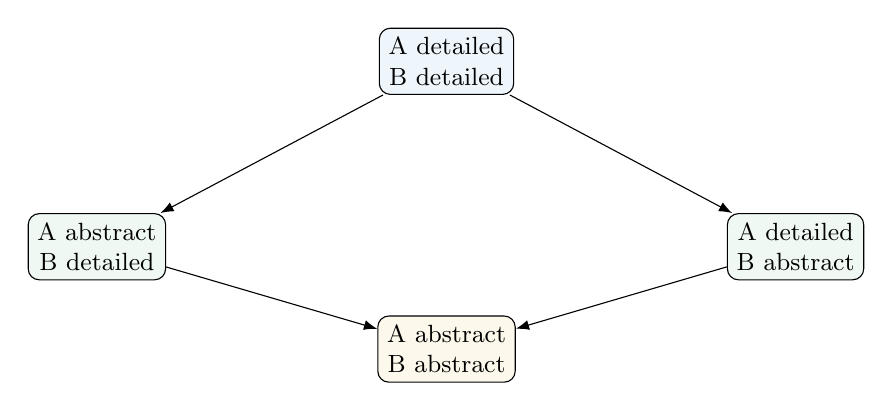
\begin{tikzpicture}[>=Latex,node distance=15mm and 27mm,every node/.style={font=\small,align=center}]
\node[draw,rounded corners,fill=sky] (fine) {A detailed\\B detailed};
\node[draw,rounded corners,fill=mint,below left=of fine] (ab) {A abstract\\B detailed};
\node[draw,rounded corners,fill=mint,below right=of fine] (ba) {A detailed\\B abstract};
\node[draw,rounded corners,fill=sand,below=28mm of fine] (coarse) {A abstract\\B abstract};
\draw[->] (fine) -- (ab);
\draw[->] (fine) -- (ba);
\draw[->] (ab) -- (coarse);
\draw[->] (ba) -- (coarse);
\end{tikzpicture}
\end{center}

\failure The two middle descriptions are incomparable. Neither is simply ``more detailed'' than the other. One keeps information about $A$ that the other discards; the other keeps information about $B$ that the first discards.

Therefore a global scalar called ``the level of granularity'' is misleading.

\lesson Computational abstractions form a \textbf{partially ordered family} under refinement. In sufficiently regular cases this family can have lattice-like structure: common refinements, common coarse-grainings, and many incomparable branches.

\begin{conceptbox}
Granularity is closer to a structured vector than to a scalar. More precisely, \textbf{abstraction is structured information loss}: what matters is not how much detail is discarded, but which distinctions are discarded.
\end{conceptbox}
\end{thoughtbox}

\begin{thoughtbox}{The stone that allegedly factors a number}
\scene Hand someone a huge semiprime and a stone. Suppose they claim that, with a sufficiently ingenious interpretation of the stone's changing microstate, the stone is performing the factorization.

The challenge is simple: identify where the input is represented, where the intermediate factors or arithmetic quantities are represented, how later physical events actually depend on earlier carriers, and where the output can be read without placing the factorization itself inside the decoding dictionary.

\failure A global state-labeling map can always hide arbitrary work in the interpretation. But that does not show that the relevant arithmetic organization occurred inside the physical process.

\lesson The actual-run notion must preserve \textbf{locality, provenance, value flow, component reuse, and causal decomposition}. It must also use a coherent representation scheme for values. An admissible computational interpretation cannot obtain its structure solely by giving each whole-system snapshot an arbitrary name or by changing the decoding rule opportunistically from one event to the next.

\begin{cautionbox}
This does not prove that a stone realizes no computations. A sufficiently rich physical episode may genuinely contain computational patterns. The claim is narrower: if a computation is present, it must be witnessed by structure in the episode itself rather than by retrospective global relabeling.
\end{cautionbox}
\end{thoughtbox}

\begin{thoughtbox}{Participation, contribution, and value support}
\scene Consider a three-input OR component. In one actual occurrence it receives
\begin{center}
\texttt{true, true, false} $\longrightarrow$ \texttt{true}.
\end{center}
All three input signals physically arrive at the component. Should the occurrent computational structure contain all three inputs? Yes, if the relation means that a value token was actually supplied as an operand. But that is not yet the same as saying that each token was important to the particular output value.

There is a useful stronger notion. Relative to the operation OR and to this actual input tuple, a \textbf{value support} for the observed output is a subset of the actual input-value assignments that is sufficient to fix that output while the remaining inputs are left unspecified. Here either \texttt{input 1 = true} alone or \texttt{input 2 = true} alone suffices to guarantee the output \texttt{true}; \texttt{input 3 = false} does not. The two true inputs therefore form two alternative minimal supports.

For an AND gate receiving \texttt{true, true}, by contrast, the observed output \texttt{true} has one joint minimal support containing both true inputs. For an XOR gate, fixing the parity result generally requires a different support pattern again.

\failure A single edge relation cannot carry all of this information. At least four questions have been mixed together:
\begin{itemize}
  \item Which tokens actually arrived and participated in the event?
  \item Which actual-value subsets are sufficient to support the particular output value?
  \item Which particular values count as causes or contributors under some theory of actual causation?
  \item Which input positions can affect the operation across alternative cases?
\end{itemize}
The first question is directly occurrent. The fourth is fully modal. The second is anchored to an actual occurrence but uses the local operation semantics to quantify over alternatives for the unspecified inputs; it is therefore \textbf{occurrence-indexed but locally modal}. The third is a further explanatory notion and is delicate under redundancy and overdetermination.

\lesson The base occurrent object should record \textbf{provenance and participation}. It may be enriched by a \textbf{value-support hypergraph}: for each actually produced value, record its minimal sufficient sets of actual value tokens relative to the local operation semantics. Actual contribution and full modal dependence should remain separate notions.

\begin{conceptbox}
Keep four structures distinct:\\[1mm]
\textbf{Participation / provenance:} this token was actually transported to, consumed by, or produced by this event.\\
\textbf{Value support:} this set of actual value assignments is sufficient to fix this actual result, relative to the local operation semantics.\\
\textbf{Actual contribution:} this actual value counts as a cause or contributor to this result under an explicit contribution criterion.\\
\textbf{Modal dependence:} this variable or port can affect the operation across admissible alternative cases.
\end{conceptbox}

\begin{cautionbox}
A value-support structure is not purely non-counterfactual. It is indexed by an actual occurrence, but sufficiency is assessed using the local rule of the operation. This makes support useful for analyzing how a result is organized without pretending that it belongs to the same ontological layer as raw provenance.
\end{cautionbox}
\end{thoughtbox}

\begin{thoughtbox}{A result produced by silence or inhibition}
\scene A downstream event occurs only if no veto signal arrives during a fixed interval. In another system, a low-voltage token explicitly carrying the Boolean value \texttt{false} arrives at a port. Both cases may be described informally as ``false,'' but their physical provenance differs: one contains a value-bearing token, while the other depends on a non-occurrence over time.

\failure A graph containing only positive event and token occurrences cannot represent absence merely by omitting a node: omission is indistinguishable from an incomplete observation or an arbitrarily cropped episode. Reifying every silence as a token also begs the question of which interval and which missing event make that token legitimate.

\lesson The base formalism is adequate for positive value flow but not universal. Applications involving inhibition, prevention, timeouts, or alternative enabling need explicit temporal windows and absence/enabling structure, or a translation into such structure whose admissibility is independently justified.
\end{thoughtbox}

\begin{thoughtbox}{One actual run does not identify the whole mechanism}
\scene Observe a component three times. On the three input cases that actually occur, its outputs agree with an AND gate. The fourth input case never occurs.

Or observe a brain for one minute in perfect detail. Suppose we know every actual computational dependency that occurred during that minute, but the subject never encountered millions of other possible sensory inputs.

\failure From the actual episode alone, we cannot infer every unrealized transition. Many distinct mechanisms may agree perfectly on everything that occurred and diverge only on cases that did not occur.

If we insist that every statement about computation must already include all these unrealized cases, then the computational identity of an actual episode becomes immediately counterfactual. If we refuse all counterfactual structure, we should not pretend that the actual run uniquely determines the full mechanism.

\lesson Split the theory into two legitimate notions.

\begin{conceptbox}
\textbf{Occurrent computation} asks what computational organization was actually instantiated in this episode.\\[1mm]
\textbf{Modal computation} asks what computational mechanism the system implements across the relevant alternative inputs and interventions.
\end{conceptbox}

The occurrent notion deliberately concludes less. It is stronger than a state trajectory because it contains actual represented provenance and composition, but weaker than a complete modal mechanism because it leaves unvisited cases open.
\end{thoughtbox}

\begin{thoughtbox}{The same realized path under different probabilities}
\scene Two stochastic mechanisms produce exactly the same finite event-token episode. Under the first mechanism the observed path had probability $0.9$; under the second it had probability $10^{-30}$ and occurred by extraordinary luck.

\failure Path identity alone does not determine whether the transition kernels belong to the identity of the computation. Conversely, kernel identity alone forgets which sample path actually occurred. Treating probability as either automatically occurrent or automatically irrelevant collapses two different questions.

\lesson A stochastic extension needs both a realized occurrence and a modal probability kernel. It must state separately whether probabilities help individuate the represented mechanism and whether a particular comparison is about the actual path, the capacity distribution, or both.
\end{thoughtbox}

\begin{thoughtbox}{Two different computers running ``the same thing''}
\scene Take two old PCs from different manufacturers. Their transistor layouts differ, their low-level timings differ, perhaps parts of their architecture differ, yet both run Windows 95 and behave similarly at familiar software interfaces.

\failure It would be wrong to say that their entire computational organization is identical. It would also be wrong to say that they share nothing computationally simply because their hardware is different.

Moreover, ``Windows 95'' itself is not a mathematically complete specification of one abstract computation. It is also the name of a historical software artifact, with versions, binaries, provenance, and conventions about what counts as the same software.

\lesson Two systems can share a large \textbf{common region of computational structure} without having identical spectra. Ordinary names such as ``the same program'' may designate some part of that common structure, but the artifact-identity question is not identical to the computational-identity question.

\begin{conceptbox}
The useful primitive comparison is not merely ``same computation: yes or no.'' It is: \textbf{what computational structure do the two systems share, and how does that shared structure sit inside each spectrum?}
\end{conceptbox}
\end{thoughtbox}

\begin{thoughtbox}{The giant lookup-table replica}
\scene Model an open synchronous system by a global transition rule: current internal state plus current input determines the next internal state and current output. Now imagine two realizations of exactly the same global rule.

One is a richly factored mechanism with many reusable local computations. The other is an enormous lookup table with one stored answer for every possible state-input pair.

\failure At the level of the global transition function, they are identical. Yet their fine internal spectra may overlap very little. The table preserves the global transduction while destroying most of the original factorization into local subcomputations.

This shows again that global functional equivalence is much weaker than fine computational equivalence.

\lesson Resource constraints create a new question. A huge table can avoid exploiting internal structure by paying with memory. As available resources are restricted, some factorizations may become unavoidable -- although compression alone does not guarantee recovery of the original factorization.

\begin{conceptbox}
This suggests a third, optional axis of the theory: \textbf{resource-constrained computational rigidity}. Among all realizations of the same abstract computation that satisfy a resource budget, which computational substructures occur in every realization?
\end{conceptbox}
\end{thoughtbox}

\section{Assembling the model}

The thought experiments above are not independent curiosities. They force a compact architecture. The theory needs only a few kinds of objects, but it must keep them separate.

\subsection{Physical episodes and computational provenance}

A \textbf{physical episode} is a bounded piece of the actual evolution of a physical system. For computational purposes, the episode should not be reduced to a sequence of global snapshots. What matters is its internal actual organization: events, typed and port-labeled value-bearing carriers or tokens, transport, consumption, production, routing, persistent component identity, control, reuse, declared boundaries, and partial order.

Call this enriched object the episode's \textbf{actual valued computational provenance structure}. The word ``provenance'' is deliberate. The base object records how pieces of represented information actually moved through and were transformed by the episode. It does not silently identify that factual participation relation with a stronger theory of which values were the decisive causes of each result.

Values require a representation discipline. The theory should not require one unique encoding for the entire physical system: the same abstract Boolean may be electrical in one subsystem, optical in another, and magnetic in a third. What it requires is a \textbf{coherent representation scheme}: a stable family of local or typed decoding rules, together with explicit translations where necessary. The scheme must be reusable across occurrences and cannot be selected separately for each point after inspecting the completed history. Context-dependent encodings are allowed when the context and translation rule are themselves part of the represented organization.

This requirement blocks a local version of the relabeling trick. A physical difference counts as a represented computational value only through a representation rule that has some stable domain of application; the decoder cannot smuggle the desired computation into a trajectory-indexed dictionary.

Repeated uses of the same component can reveal more structure without introducing global counterfactual commitments. If the component is actually observed on several input tuples, the episode may support a \textbf{partial operation table}: what that component in fact did on the cases that occurred. Unvisited input tuples remain unspecified at the occurrent level.

A second enrichment is possible when the local operation type is independently available. For one actual operation occurrence, define a \textbf{value support} as a set of actual input-value assignments sufficient to fix the actual output value while the remaining inputs are left free. Minimal supports form a hypergraph over the actual value tokens. This object is useful but must be classified carefully: it is anchored to an actual occurrence yet uses local modal semantics to test sufficiency. It is therefore richer than provenance and weaker than importing the modal organization of the whole system.

\begin{definitionbox}
An \textbf{occurrent computational abstraction} is a structure-preserving compression of an actual valued computational provenance structure under a coherent representation scheme. It may hide internal details, merge events, or replace a detailed subsystem by an abstract component, but every retained operand, result, dependency, and precedence relation must have an actual witness. Selecting a subepisode must either retain a selected event's relevant incident tokens or expose them explicitly at its boundary.
\end{definitionbox}

\subsection{Four relations that should not be collapsed}

The phrase ``causal structure'' is too overloaded to serve as a single primitive. At least four relations should be kept conceptually separate.

\begin{center}
\begin{tabularx}{\textwidth}{>{\RaggedRight\arraybackslash\bfseries}p{33mm}>{\RaggedRight\arraybackslash}X>{\RaggedRight\arraybackslash}X}
\toprule
Relation & What it says & Modal status \\
\midrule
Participation / provenance & A token was actually delivered to, consumed by, transported through, or produced by an event & Strictly occurrent base relation \\
Value support & A set of actual input-value assignments is sufficient for the actual result relative to the local operation semantics & Occurrence-indexed, locally modal \\
Actual contribution & A particular actual value contributed to a particular actual result under an explicit theory of actual causation or contribution & Optional explanatory enrichment \\
Modal dependence & An input, variable, or component can affect another across admissible alternative cases & Fully modal mechanism relation \\
\bottomrule
\end{tabularx}
\end{center}

The distinctions matter even for tiny examples. In \texttt{OR(true,true,false)=true}, all three tokens participate, the false token belongs to no minimal sufficient support for the true output, and the two true tokens appear as alternative minimal supports. Yet all three ports belong to the gate's modal dependence structure. A theory of actual causation may classify the two redundant true values in still another way.

The support relation is naturally hypergraphic rather than merely graphical. An AND output may require a joint set of values; an OR output may have several alternative singleton supports. Keeping this structure separate prevents the theory from pretending that one binary edge relation captures participation, sufficiency, explanatory contribution, and counterfactual dependence at once.

\subsection{Modal mechanisms}

A \textbf{modal computational mechanism} enriches the actual organization with stable rules across a relevant family of possible inputs and interventions. It says not only how one episode unfolded, but how the same organization would transform other admissible states or respond to perturbations.

Modal structure is what distinguishes an actual partial regularity from a full implemented rule. The component observed on three AND-compatible cases may support an occurrent partial operation; calling it an AND gate in the full mechanistic sense requires the missing modal commitment.

\begin{definitionbox}
A \textbf{modal computational abstraction} is an admissible abstraction of a physical mechanism that preserves the computational organization across the relevant alternatives, not merely along one realized history.
\end{definitionbox}

\subsection{The computational spectrum}

A system should not be assigned one privileged computational level. It supports many admissible abstractions, often incomparable because different subsystems can be abstracted independently.

The structured family of these abstractions is its \textbf{computational spectrum}.

For one actual episode we obtain an \textbf{occurrent computational spectrum}. For the underlying mechanism we obtain a \textbf{modal computational spectrum}.

Schematic notation is useful even in an informal account:
\[
\mathrm{Spec}_{\mathrm{occ}}(E),
\qquad
\mathrm{Spec}_{\mathrm{mod}}(M).
\]

These are not merely unstructured bags of descriptions. They carry at least a refinement relation: one member refines another when it preserves every distinction retained by the coarser member and adds further structure.

\begin{thesisbox}[title={Implementation without an observer-selected level}]
A physical system implements an abstract computation $C$ when $C$ occurs as an admissible member of the relevant computational spectrum.

The observer may decide to ask about $C$, but does not create $C$ by selecting a level. More exactly, relative to a carrier, factorization, and decoder policy fixed independently of $C$, the system either contains the required structure or it does not. Different scientific domains may justify different policies; hiding that parameter would overstate the objectivity claim.
\end{thesisbox}

\subsection{Why there are two spectra}

The occurrent and modal spectra answer different questions.

\begin{center}
\begin{tabularx}{\textwidth}{>{\RaggedRight\arraybackslash\bfseries}p{28mm}>{\RaggedRight\arraybackslash}X>{\RaggedRight\arraybackslash}X}
\toprule
 & Occurrent spectrum & Modal spectrum \\
\midrule
Target & One actual episode & The stable mechanism \\
Contains & Actual events, represented values, participation/provenance, partial operations, local composition; optionally value supports when local operation semantics are supplied & Transition organization and modal dependence across relevant inputs and interventions \\
Strength & Weaker & Stronger \\
Leaves open & Unvisited cases & Nothing inside the specified modal domain \\
Blocks & Mere relabeling of snapshots & Accidental agreement on one history \\
\bottomrule
\end{tabularx}
\end{center}

A modal realization whose variable grouping is backed by local event and port witnesses, when actually executed, should produce a corresponding occurrent realization under the same representation scheme. Global state-transition agreement alone is insufficient, because two mechanisms with the same global transition can have different internal provenance. A single occurrent realization generally admits many possible modal completions. The occurrent trace can constrain those completions by accumulating partial operation tables without selecting values for cases that never occurred.

This relationship can be pictured without implying that abstraction and modality are the same dimension:

\begin{center}
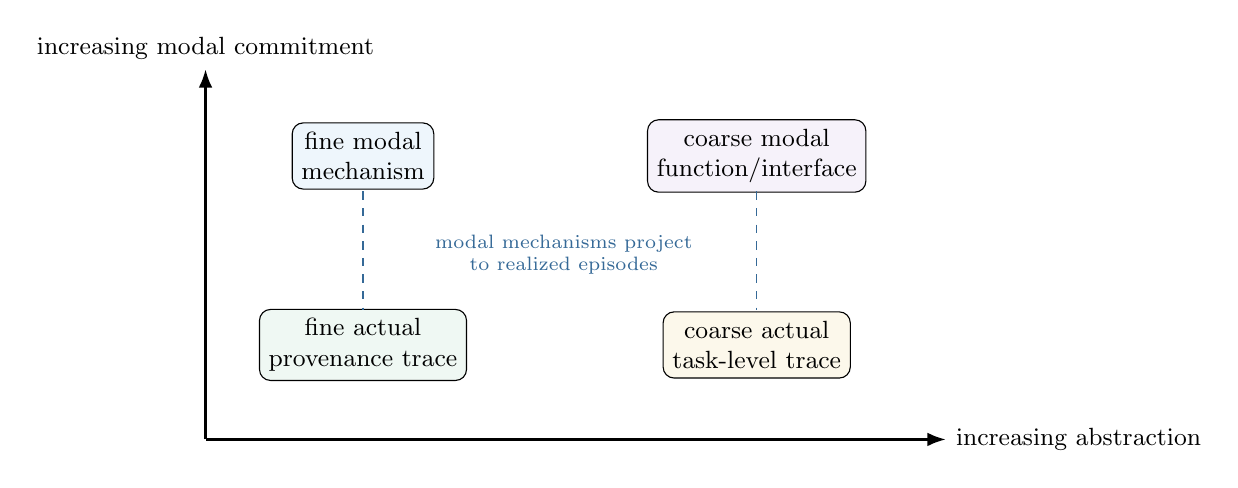
\begin{tikzpicture}[>=Latex,every node/.style={font=\small}]
\draw[->,thick] (0,0) -- (9.4,0) node[right]{\small increasing abstraction};
\draw[->,thick] (0,0) -- (0,4.7) node[above]{\small increasing modal commitment};
\node[draw,rounded corners,fill=mint,align=center] at (2.0,1.2) {fine actual\\provenance trace};
\node[draw,rounded corners,fill=sand,align=center] at (7.0,1.2) {coarse actual\\task-level trace};
\node[draw,rounded corners,fill=sky,align=center] at (2.0,3.6) {fine modal\\mechanism};
\node[draw,rounded corners,fill=violet,align=center] at (7.0,3.6) {coarse modal\\function/interface};
\draw[dashed,blue] (2.0,3.15) -- (2.0,1.65);
\draw[dashed,blue] (7.0,3.15) -- (7.0,1.65);
\node[font=\scriptsize,blue,align=center] at (4.55,2.35) {modal mechanisms project\\to realized episodes};
\end{tikzpicture}
\end{center}

\section{The internal geometry of a computational spectrum}

Once the spectrum replaces the picture of one privileged level, several comparative notions become natural.

\subsection{Refinement}

A computation $A$ \textbf{refines} a computation $B$ when there is an admissible abstraction from $A$ to $B$. Before quotienting, this relation is generally only a preorder: two non-identical descriptions may abstract to one another. The spectrum becomes a partial order after identifying mutual-abstraction classes. Replacing a loop by a black-box ``SUM'' component moves from a finer member of the spectrum to a coarser one. Abstracting a different component gives a different branch, not necessarily a higher or lower point on one scalar ladder.

\subsection{Containment}

A system $X$ has \textbf{computational containment} over $Y$ when the relevant computational structure of $Y$ embeds into the spectrum of $X$. Schematically one may write
\[
\mathrm{Spec}(Y) \hookrightarrow \mathrm{Spec}(X),
\]
with the understanding that the embedding should respect refinement relations, not merely set membership.

Emulation is a natural source of containment: a richer system may realize the computational organization of another system while also realizing additional structures.

\subsection{Computational equivalence}

Two systems are \textbf{spectrally equivalent} in a strong sense when their relevant computational spectra have the same structure. This is much stronger than saying that they compute the same input-output function or run the same software artifact.

Strong spectral equivalence is therefore not the default notion of ``same computation.'' It is one precise endpoint in a family of comparisons.

\subsection{Common computational core}

The most useful comparison between different systems is often their \textbf{common computational core}: the structured family of computational abstractions realized by both.

For systems $X$ and $Y$, the informal idea is the structured overlap
\[
\mathrm{Core}(X,Y) \sim \mathrm{Spec}(X) \cap \mathrm{Spec}(Y).
\]

The notation hides technical choices about isomorphism and embedding, but the concept is clear: two machines can be deeply different while still sharing a rich common computational organization.

Every spectrum may also contain trivial bottom abstractions. Their presence in every intersection is not evidence of a substantive common core. Comparisons should therefore identify maximal nontrivial common elements, impose a rank or resource baseline, or explicitly subtract the universal bottom structure.

\begin{takeawaybox}
The question ``are these two machines doing the same computation?'' is usually underspecified. Better questions are:
\begin{itemize}
  \item Which computations occur in both spectra?
  \item Does one spectrum contain a faithful copy of part of the other?
  \item What is the richest common abstraction?
  \item At which refinements do the systems diverge?
\end{itemize}
\end{takeawaybox}

\section{Objectivity, context, and naming}

The theory separates three issues that are often collapsed.

\textbf{First: physical realization.} Once a realization policy has been fixed independently of the target computation, whether an admissible structure occurs in the spectrum is intended to be an objective fact about the system. Admissibility includes coherent representation, boundary fullness, and provenance witnessing: a computational value or dependency cannot be rescued by changing the codebook opportunistically or by drawing an abstract edge with no physical witness.

\textbf{Second: abstraction.} The spectrum contains many abstractions at once. No single member has to be privileged as ``the'' computational level.

\textbf{Third: reference.} Human language may be vague about which abstract object is intended. ``Windows 95,'' ``the same algorithm,'' or ``the same agent'' can underdetermine what part of the spectrum is being named.

This locates some conventionality in the question rather than in the physical realization. A name may fail to specify its target precisely; that does not imply that membership in a policy-indexed spectrum is observer-relative. The stronger claim that one admissibility policy is uniquely privileged across all scientific domains is neither needed nor established here.

Context also matters locally. Two subroutines can be interchangeable for a caller that sees only input and output, yet distinguishable for a caller that observes timing, intermediate memory, power use, or interruptibility. The admissible abstraction must therefore preserve every distinction that remains accessible through the interface of the larger computation.

\section{Consequences that fall out of the model}

The model is informal here, but several theorem-like consequences follow almost immediately from the architecture.

\begin{consequencebox}[title={1. Bare trajectory identity is too weak}]
If computational identity preserves only temporal succession of atomic global states, trivial relabelings are unavoidable. Any nontrivial occurrent notion must preserve more internal structure than a state sequence.
\end{consequencebox}

\begin{consequencebox}[title={2. Value identity requires a coherent representation scheme}]
An occurrent implementation cannot be certified by a decoder that changes opportunistically along the trajectory. Representation may be heterogeneous across physical subsystems, but each local or typed code must be stable enough to be reused across occurrences without consulting the completed run.
\end{consequencebox}

\begin{consequencebox}[title={3. Participation, support, contribution, and modal dependence are different}]
A value can be an actual operand without belonging to any minimal support of the observed result; a minimal support can be one among several redundant alternatives; an actual-causation criterion can classify those alternatives differently; and a port can belong to the modal dependence structure even when its current token is support-irrelevant. These relations should not be collapsed into one causal edge.
\end{consequencebox}

\begin{consequencebox}[title={4. Value support is intermediate rather than purely occurrent}]
Minimal sufficient supports are indexed by an actual event and actual values, but their sufficiency is evaluated using the local operation semantics over unfilled inputs. They are therefore a principled intermediate object between raw provenance and full-system modal structure.
\end{consequencebox}

\begin{consequencebox}[title={5. Function identity is a quotient, not full identity}]
Distinct computations can collapse to the same input-output function. Therefore equality of functions can be recovered as a coarse spectral equivalence without being mistaken for equality of finer algorithms.
\end{consequencebox}

\begin{consequencebox}[title={6. Abstraction is generally only partially ordered}]
Independent local abstractions generate incomparable descriptions. Existence of an abstraction first gives a preorder; quotienting descriptions that abstract to one another gives the corresponding partial order. A theory that represents granularity by one scalar level discards real structure in the space of computational descriptions.
\end{consequencebox}

\begin{consequencebox}[title={7. Modal realization projects to occurrent realization}]
Whenever a modal realization is backed by compatible local event and port witnesses and is actually run, the realized episode instantiates a compatible occurrent member. Commutation of global states alone does not establish this projection.
\end{consequencebox}

\begin{consequencebox}[title={8. Occurrent realization underdetermines modal realization}]
Even a complete actual provenance structure need not determine what would have happened in unvisited cases. One occurrent spectrum can therefore be compatible with many modal completions.
\end{consequencebox}

\begin{consequencebox}[title={9. Local substitution is controlled by interface}]
If a context can observe only an abstract interface of a subsystem, implementations that are equivalent at that interface may be substituted without changing the coarser surrounding computation. If the context observes additional distinctions, the substitution may cease to be valid.
\end{consequencebox}

\begin{consequencebox}[title={10. ``Same computation'' is naturally many-valued in structure, not vague in truth}]
Two systems may share one computation, many computations, or an entire common subspectrum while differing elsewhere. The richness of shared structure replaces a single primitive yes/no relation.
\end{consequencebox}

\begin{consequencebox}[title={11. Occurrent repetition can reveal partial laws without becoming modal}]
If the same component is actually encountered on several input cases, the occurrent structure can accumulate a partial operation table. This can strongly constrain compatible modal mechanisms while leaving unvisited cases genuinely open. More observation can therefore enrich occurrent computation without erasing the occurrent/modal distinction.
\end{consequencebox}

\begin{consequencebox}[title={12. Resource restriction can enlarge the inevitable common core}]
Fix an abstract computation and consider all of its admissible realizations satisfying a resource budget. Intersect their spectra. If the budget is tightened, the class of admissible realizations shrinks, so this inevitable common core can only stay the same or grow.

This does \emph{not} imply that stronger compression always recovers the architecture of some chosen original system. Different compact algorithms may still exist. It instead defines a clean notion of \textbf{computational rigidity}: which structures become unavoidable under resource pressure.

Trivial bottom abstractions should be removed or discounted when reporting such a core; otherwise every intersection can look nonempty for an uninformative reason.
\end{consequencebox}

\section{A compact reconstruction of the theory}

The formal theory can be reconstructed from this note in the following order.

\begin{enumerate}
  \item \textbf{Represent actual processes richly.} Use typed ports, events, value-bearing tokens, persistent component identities, declared boundaries, actual transport, consumption, production, ordering, control, reuse, and composition. Do not begin from atomic state sequences.
  \item \textbf{Fix coherent value representation and admissibility.} Allow heterogeneous local encodings, but require stable typed decoding rules and explicit translations. Fix the eligible carriers and decoder family independently of the desired trajectory; stationarity alone is insufficient when every exact carrier state is unique.
  \item \textbf{Separate dependence relations.} Use participation/provenance as the base occurrent relation. Distinguish it from actual contribution and from general modal dependence.
  \item \textbf{Add value support only as an explicit enrichment.} When local operation semantics are supplied, actual values can be organized into minimal sufficient support sets. Record that this is occurrence-indexed but locally modal, not primitive provenance.
  \item \textbf{Define admissible abstractions.} An abstraction may forget internal distinctions only when every retained incidence, dependency, and boundary relation has a physical witness.
  \item \textbf{Order abstractions by refinement.} Allow different subsystems to be abstracted independently, first obtaining a preorder and then its poset reflection; lattice-like structure requires further conditions.
  \item \textbf{Build the occurrent spectrum.} For a physical episode, collect all admissible abstractions of its actual valued computational provenance structure. Repeated actual cases may determine partial operation tables.
  \item \textbf{Build the modal spectrum.} For a mechanism, collect all admissible abstractions whose transition organization and dependence structure remain valid across the relevant alternative inputs and interventions.
  \item \textbf{Relate the two locally.} Unfolding-compatible modal structures project to actual runs; actual runs and their partial laws constrain but generally do not uniquely determine modal completions.
  \item \textbf{Define implementation by membership.} A computation is implemented when it occurs in the relevant spectrum, not because an observer has privileged a level.
  \item \textbf{Compare systems spectrally.} Use refinement, containment, spectral equivalence, and common computational core rather than one undifferentiated relation of sameness.
  \item \textbf{Keep naming separate.} Artifact labels such as program names may require additional historical or conventional criteria beyond computational structure.
  \item \textbf{Optionally add resource constraints.} Study how the common core of all realizations changes as memory, description length, time, circuit size, locality, or other resources are restricted.
\end{enumerate}

\begin{thesisbox}[title={The final picture}]
The theory has two primary axes and one optional third axis.

\textbf{Abstraction axis:} which distinctions in the computation are retained? This produces a branching refinement structure rather than one scalar level.

\textbf{Modal axis:} are we describing only represented value flow, participation, and provenance actually instantiated; enriching that occurrence with local support information; or describing the full transition and dependence mechanism across unrealized alternatives?

\textbf{Resource axis:} among all realizations of the same abstract computation, which internal structures become unavoidable when the admissible resource region contracts?

The resulting object is not ``the computation of the system'' but a structured computational spectrum. Objective implementation becomes spectrum membership; similarity between systems becomes structured overlap; coherent representation and provenance block arbitrary trajectory relabeling at the occurrent level; and the occurrent/modal distinction separates what actually happened from the stronger mechanism across unrealized alternatives.
\end{thesisbox}


\section{From computational identity to computational functionalism}

The preceding sections develop an ontology of computational realization in terms of actual episodes, modal mechanisms, and structured spectra of abstraction. That ontology provides the basis for a distinct question:

\begin{center}
\textbf{What structural constraints should any consciousness-making computational property satisfy?}
\end{center}

The aim is to constrain the architecture of computational-functionalist theories; the substantive theory supplies the neural or algorithmic property that bears consciousness.

\subsection{The primary bearer should be an episode, not an abstract program}

An abstract algorithm is a type. It can be instantiated zero, one, or many times. A conscious experience, by contrast, is naturally treated as an occurrence: something happening in a particular system over a particular interval.

A computational functionalism should therefore assign phenomenal properties primarily to \textbf{actually instantiated computational episodes}, or to equivalence classes of such episodes under a family of neutral redescriptions specified independently of the phenomenal verdict. The modal computational spectrum remains important for what the system can do, but it need not be constitutive of what is experienced in one actual episode.

\begin{principlebox}[title={Phenomenal Actuality}]
The phenomenal character of an episode should supervene on properties of the computational process actually instantiated in that episode. No phenomenal difference should arise from a difference that exists only outside the actual process, unless the theory explicitly argues that the modal difference itself is consciousness-relevant.
\end{principlebox}

\subsection{Counterfactual differences should not matter by themselves}

Suppose every actually encountered instance of a two-input OR gate has input \texttt{true,true} and output \texttt{true}. Replace those gates by AND gates. On the episode that actually occurs, the same tokens arrive and the same output tokens are generated in the same larger provenance pattern. The two mechanisms differ sharply on \texttt{true,false}, but that case never occurs.

A theory that changes the present phenomenology merely because the replacement gate \emph{would have} behaved differently on an unencountered input is making current experience depend on an unrealized branch. That may be a coherent metaphysical position, but it carries a substantial and unnecessary commitment.

\begin{principlebox}[title={Counterfactual Irrelevance}]
After the actual computational structure has been independently grounded, differences confined to unrealized alternatives and playing no role in individuating its carriers, events, representations, boundaries, or actual dependencies should not, by themselves, constitute phenomenal differences in the episode.
\end{principlebox}

This principle is stronger than merely saying that the system's observable input-output behavior is the same. The actual internal generative process may still matter. But the qualification is essential because modal information can play three different roles:

\begin{enumerate}
  \item \textbf{Individuating:} dispositions may help determine which carriers, operations, component identities, or representations are present in the actual episode.
  \item \textbf{Evidential:} interventions may reveal which actual dependencies and boundaries the system possesses.
  \item \textbf{Constitutive:} unmanifested alternatives may themselves be proposed as part of the present phenomenal basis.
\end{enumerate}

Counterfactual Irrelevance rejects the automatic move in the third role. It does not ban the first two, and it cannot be used to validate an arbitrary actual-run decoding whose grounding already fails.

\begin{stressbox}[title={OR versus AND: why value support should not automatically be phenomenal}]
For \texttt{OR(true,true)=true}, the actual output has two alternative singleton minimal supports. For \texttt{AND(true,true)=true}, it has one joint support containing both inputs. Thus the value-support hypergraphs differ even though the actual token flow and generated values can be identical.

This is exactly why value support belongs in the theory of computation but should \emph{not} automatically be declared consciousness-constitutive. Its difference here is obtained from local counterfactual semantics. A candidate consciousness theory may use support structure if it has an independent reason to do so, but support difference alone should not be treated as an automatic phenomenal difference.
\end{stressbox}

\begin{stressbox}[title={Dormant error correction: an individuation test}]
Suppose the same actual bit sequence passes through two devices, but only one belongs to an error-correcting architecture. No error occurs during the episode. The dormant code need not contribute directly to present phenomenology; nevertheless, it may help determine what counts as a bit, an error, a component boundary, or a correction operation. This case separates a modal fact used to individuate the actual computation from a modal fact promoted to a phenomenal constituent.
\end{stressbox}

\subsection{Actual generation should matter more than snapshot succession}

Counterfactual irrelevance does not imply that any replay of the same sequence of states is equivalent. A movie player can display a sequence of recorded brain states while each frame is produced by reading storage rather than by the preceding computational organization. The state sequence can match while the actual provenance of value production does not.

\begin{principlebox}[title={Generative-Process Sensitivity}]
A computational functionalism may legitimately depend on how the actual episode is generated: which represented values are produced, transmitted, combined, and reused by which actual events. Equality of snapshots or output traces alone is too weak.
\end{principlebox}

This gives a middle position. It is richer than pure input-output functionalism, but less modal than requiring the entire counterfactual machine to be preserved.

\subsection{Representation, substrate, and inert structure should be irrelevant}

Several transformations should be presumptively consciousness-neutral when they leave the relevant actual computation unchanged.

\begin{principlebox}[title={Representation Invariance}]
A coherent renaming or recoding of computational values should not change phenomenology merely because a different physical or symbolic code is used.
\end{principlebox}

\begin{principlebox}[title={Substrate Invariance}]
Changing the physical material should not change phenomenology when the consciousness-relevant actual computational organization is preserved. Otherwise the theory is no longer computationally functionalist in the intended sense.
\end{principlebox}

\begin{principlebox}[title={Inert-Extension Invariance}]
Adding structure that is causally isolated from the declared bearer boundary throughout the relevant interval---not merely absent from a preferred description---should not alter the phenomenology of that episode.
\end{principlebox}

The last principle is especially important. Without it, attaching a physically inert device whose only role is to change what the system \emph{could} have done can change present experience without changing anything that actually happens.

\subsection{Redescription and harmless implementation detail should not multiply experience}

The computational spectrum contains many abstractions of one episode. A neuronal description, a circuit description, and a task-level description can all be true at once. It would be pathological to count each as a new consciousness merely because the same process admits several computational witnesses.

\begin{principlebox}[title={Abstraction Consistency}]
Each candidate theory should specify a family of neutral redescriptions and refinements using computational or physical criteria independent of the phenomenal verdict. Consciousness-making properties should be invariant under that family. Multiple spectral descriptions of one physical realization do not by themselves imply multiple phenomenal subjects or episodes.
\end{principlebox}

This principle does not solve subject individuation when genuinely distinct or overlapping subsystems each instantiate candidate consciousness-bearing structures. That is a separate problem that a complete theory must address.

\subsection{Robustness and present phenomenality should be separated}

Consider an extreme replica of one minute of brain activity. Every component is replaced by a brittle device engineered only to produce the correct outputs on the inputs it will actually encounter during that minute. The device would fail on nearby unrealized cases, but the actual generative provenance of the target episode is preserved.

An actualist computational functionalism should accept the following distinction:

\begin{itemize}
  \item the replica and the brain can differ radically in \textbf{modal robustness}, future capacity, and counterfactual competence;
  \item they can nevertheless instantiate the same \textbf{actual phenomenal episode} if the consciousness-relevant actual process is genuinely preserved.
\end{itemize}

\begin{principlebox}[title={Capacity--Occurrence Separation}]
The modal computational spectrum is the natural home of capacities: what conscious episodes a system could support, how robustly it can continue, and how it would respond to other conditions. The phenomenology of the episode currently instantiated should be grounded primarily in its occurrent computational organization.
\end{principlebox}

This avoids making present phenomenology depend on unused competence while preserving a substantial role for modal computation in the theory of conscious agents.

A stochastic variant sharpens the issue. Two systems may realize the same finite episode even though the episode is typical under one transition kernel and astronomically unlikely under the other. An actual-process theory must say whether those probabilities merely characterize capacity, help individuate the actual process, or enter phenomenology directly; the slogan ``same path'' does not decide the matter.

\subsection{A class of admissible computational-functionalist theories}

The preceding principles do not identify the consciousness-making invariant. They restrict the form of an acceptable candidate. A candidate property $P$ is structurally well behaved if it satisfies, or explicitly justifies violating, the following expectations:

\begin{enumerate}
  \item $P$ is a property of an actually instantiated computational organization, not merely of an abstract program considered without a realization.
  \item $P$ is invariant under coherent value recoding and irrelevant substrate changes.
  \item $P$ does not change merely because unrealized transition rules or structures causally isolated from the declared bearer are altered, once the actual organization has been independently individuated.
  \item $P$ can be sensitive to actual internal generation and provenance, so that a movie playback need not be equivalent to a genuine computation.
  \item $P$ is stable across an independently specified family of neutral abstractions and refinements; neutrality is not defined by presupposing $P$'s output.
  \item If $P$ depends on a locally modal object such as value support, the theory must explain why that local counterfactual information is constitutive rather than merely diagnostic.
  \item $P$ distinguishes phenomenal occurrence from modal capacity rather than treating them as the same question.
  \item $P$ states its bearer boundary and prevents multiple descriptions or overlapping quotients from automatically multiplying subjects.
  \item $P$ supplies diachronic and robustness conditions: subdivision, concatenation, timing variation, noise, and approximation have explicit effects rather than being left to the choice of description.
  \item $P$ is operationally constrainable in principle; its extraction rule cannot encode the phenomenal verdict it is meant to predict.
\end{enumerate}

\begin{thesisbox}[title={The proposed default architecture}]
A deliberately actualist form of computational functionalism is \textbf{actual-process computational functionalism}: phenomenal facts supervene on independently grounded invariants of the computation actually generated during an episode, modulo coherent recoding, substrate changes, explicitly neutral refinement, and causally isolated extensions. Modal structure can individuate mechanisms, support evidence, describe capacities, and constrain possible episodes, but a difference confined to unrealized alternatives is not by itself a difference in the phenomenology of the episode that occurred.
\end{thesisbox}

\section{Division of theoretical labor in the combined framework}

The computational theory and the functionalist constraints now play different roles.

\textbf{The computational theory} tells us, relative to an independently fixed realization policy, what structures are realized: provenance, representation, abstractions, partial operations, optional support structures, modal mechanisms, spectra, refinement, containment, and common computational cores.

\textbf{The functionalist framework} tells us how a consciousness theory should use those structures without inheriting avoidable pathologies. In particular, it warns against four shortcuts:

\begin{itemize}
  \item identifying consciousness with a bare input-output function;
  \item identifying it with a relabelable sequence of states;
  \item making it automatically sensitive to the entire counterfactual machine;
  \item treating every computational description of one process as a separate phenomenal realization.
\end{itemize}

The resulting research question is therefore sharper than ``which computation is conscious?'' It is:

\begin{center}
\textbf{Which invariants of an actually instantiated computational spectrum are phenomenal, and what additional modal information, if any, has an independent reason to be constitutive?}
\end{center}

This leaves the substantive theory of consciousness open while specifying a much narrower and more disciplined target space for such theories.

\section*{One-sentence version}

\begin{center}
\fbox{\parbox{0.91\textwidth}{\centering
\textbf{Relative to independently fixed realization policies, physical systems support structured spectra of computational abstractions grounded in coherent representation and witness-full actual provenance; modal structure strengthens this into claims about alternative cases, while a deliberately actualist computational functionalism places present phenomenology primarily on independently grounded invariants of the generated process and rejects unrealized differences as sufficient phenomenal differences unless their constitutive role is separately argued.}
}}
\end{center}

\end{document}
